\chapter{Time-dependent synced-rotational gains} % Main chapter title

\label{Chapter3} % Change X to a consecutive number; for referencing this chapter elsewhere, use \ref{ChapterX}
\section{Proposed method}
This paper proposes a strategy with a time-dependent synced-rotational gain to avoid collisions between multiple VR users sharing the same physical space. A time-dependent synced-rotational gain will rotate the coordinates of all the virtual environments as the time passes, which belong to the users in a collision course in order to have them face in a different direction to avoid collisions. Fig.~\ref{fig:Time-Dependent Synced Rotational Strategy} shows the process of the strategy. Fig.~\ref{fig:Time-Dependent Synced Rotational Strategy_a} predicts a collision from walking directions of three users and their current positions in their physical space. After the collision is predicted, Fig.~\ref{fig:Time-Dependent Synced Rotational Strategy_b} rotates the coordinates of their VR cameras counterclockwise
at the same time to change their facing direction. Fig.~\ref{fig:Time-Dependent Synced Rotational Strategy_c} shows the result of the strategy.

This strategy is expected to be better than Holm's method when more than two users sharing the same physical space because when three or more users have predicted a collision at the same time, Holm's method can enable collision avoidance function for just two users. The other user will get nothing, but our method can enable a collision avoidance function when three or more users are predicted a collision.

\begin{figure}[H]
	\centering
		\subfigure[Predict a collision.]{
			\begin{minipage}[t]{0.5\linewidth}
				\centering
				\includegraphics[width=1.9in]{Pictures/A strategy with a time-dependent synced rotational gain_1.png}
				\label{fig:Time-Dependent Synced Rotational Strategy_a}
			\end{minipage}
		}%
		\subfigure[Rotate the coordinates of the VR cameras counterclockwise that belong to users on a collision course.]{
			\begin{minipage}[t]{0.5\linewidth}
				\centering
				\includegraphics[width=1.9in]{Pictures/A strategy with a time-dependent synced rotational gain_2.png}
				\label{fig:Time-Dependent Synced Rotational Strategy_b}
			\end{minipage}
		}%

		\subfigure[Change the users' facing direction at the same time.]{
			\begin{minipage}[t]{0.5\linewidth}
				\centering
				\includegraphics[width=1.9in]{Pictures/A strategy with a time-dependent synced rotational gain_3.png}
				\label{fig:Time-Dependent Synced Rotational Strategy_c}
			\end{minipage}
		}%
	
		\centering
		\caption{A strategy with a time-dependent synced rotational gain.}
		\label{fig:Time-Dependent Synced Rotational Strategy}
\end{figure}

To make the proposed method work properly, the following two properties should be figured out prior to implementation.
\begin{enumerate}
  \item Sensitivity of rotational awareness of humans in a virtual environment
  \item Curvature distance of humans walking in a rotating virtual environment
\end{enumerate}

%%%%%%%%%%%%%%%%%%%%%%%%%%%%%%%%%%%%%%%%%%%%%%%%%%%%%%%
%Positon prediction&Walking direction prediction/Collision detection/Collision avoidance
For predicting a collision of users and detecting the collision, the proposed method implements the position prediction, walking direction prediction and collision detection from the Holm's method mentioned in the previous chapter. As for collision avoidance, the Holm's method is designed to handle between two users. If the number of users is three or more users sharing the same physical space, a collision might occur between more than two users at the same time. In that case, the exceed users from two will get nothing and are not treated as the target of collision avoidance. The proposed method can reduce the collision number when the collision occurs between more than two users.






%%%%%%%%%%%%%%%%%%%%%%%%%%%%%%%%%%%%%%%%%%%%%%%%%%%%%%%
\newpage
%%%%%%%%%%%%%%%%%%%%%%%%%%%%%%%%%%%%%%%%%%%%%%%%%%%%%%%%%%
%%%%%%%%%%%%%%%%%%%%%%%%%%%%%%%%%%%%%%%%%%%%%%%%%%%%%%%%%%	
\section{Sensitivity of rotational awareness of humans in a virtual environment}
For properties of rotation of a virtual environment, the purpose of this experiment is to figure out the threshold that humans cannot sense the applied rotation.


\subsection{Experiment tasks}
In this experiment, three tasks are employed: stop to constant speed rotation task, constant speed to stop rotation task, deceleration rotation task and acceleration rotation task. 

Fig.~\ref{fig:topView} and Fig.~\ref{fig:sideView} represent a virtual environment used in the experiment. At the beginning of tasks, the position of a user is located at the origin (0,0) on XZ plane. In the figures, the user stands at the origin. The user can see around in the virtual environment from a field of view of 110 degrees (Fig.~\ref{fig:sideView}), and the user can freely turn around in the virtual environment. 


\begin{figure}[H]\centering
	\includegraphics[width=0.95\textwidth]{Pictures/topView.png}%imagine location
	\caption{A virtual environment from top view.}\label{fig:topView}%use name for ref.
\end{figure}

\begin{figure}[H]\centering
	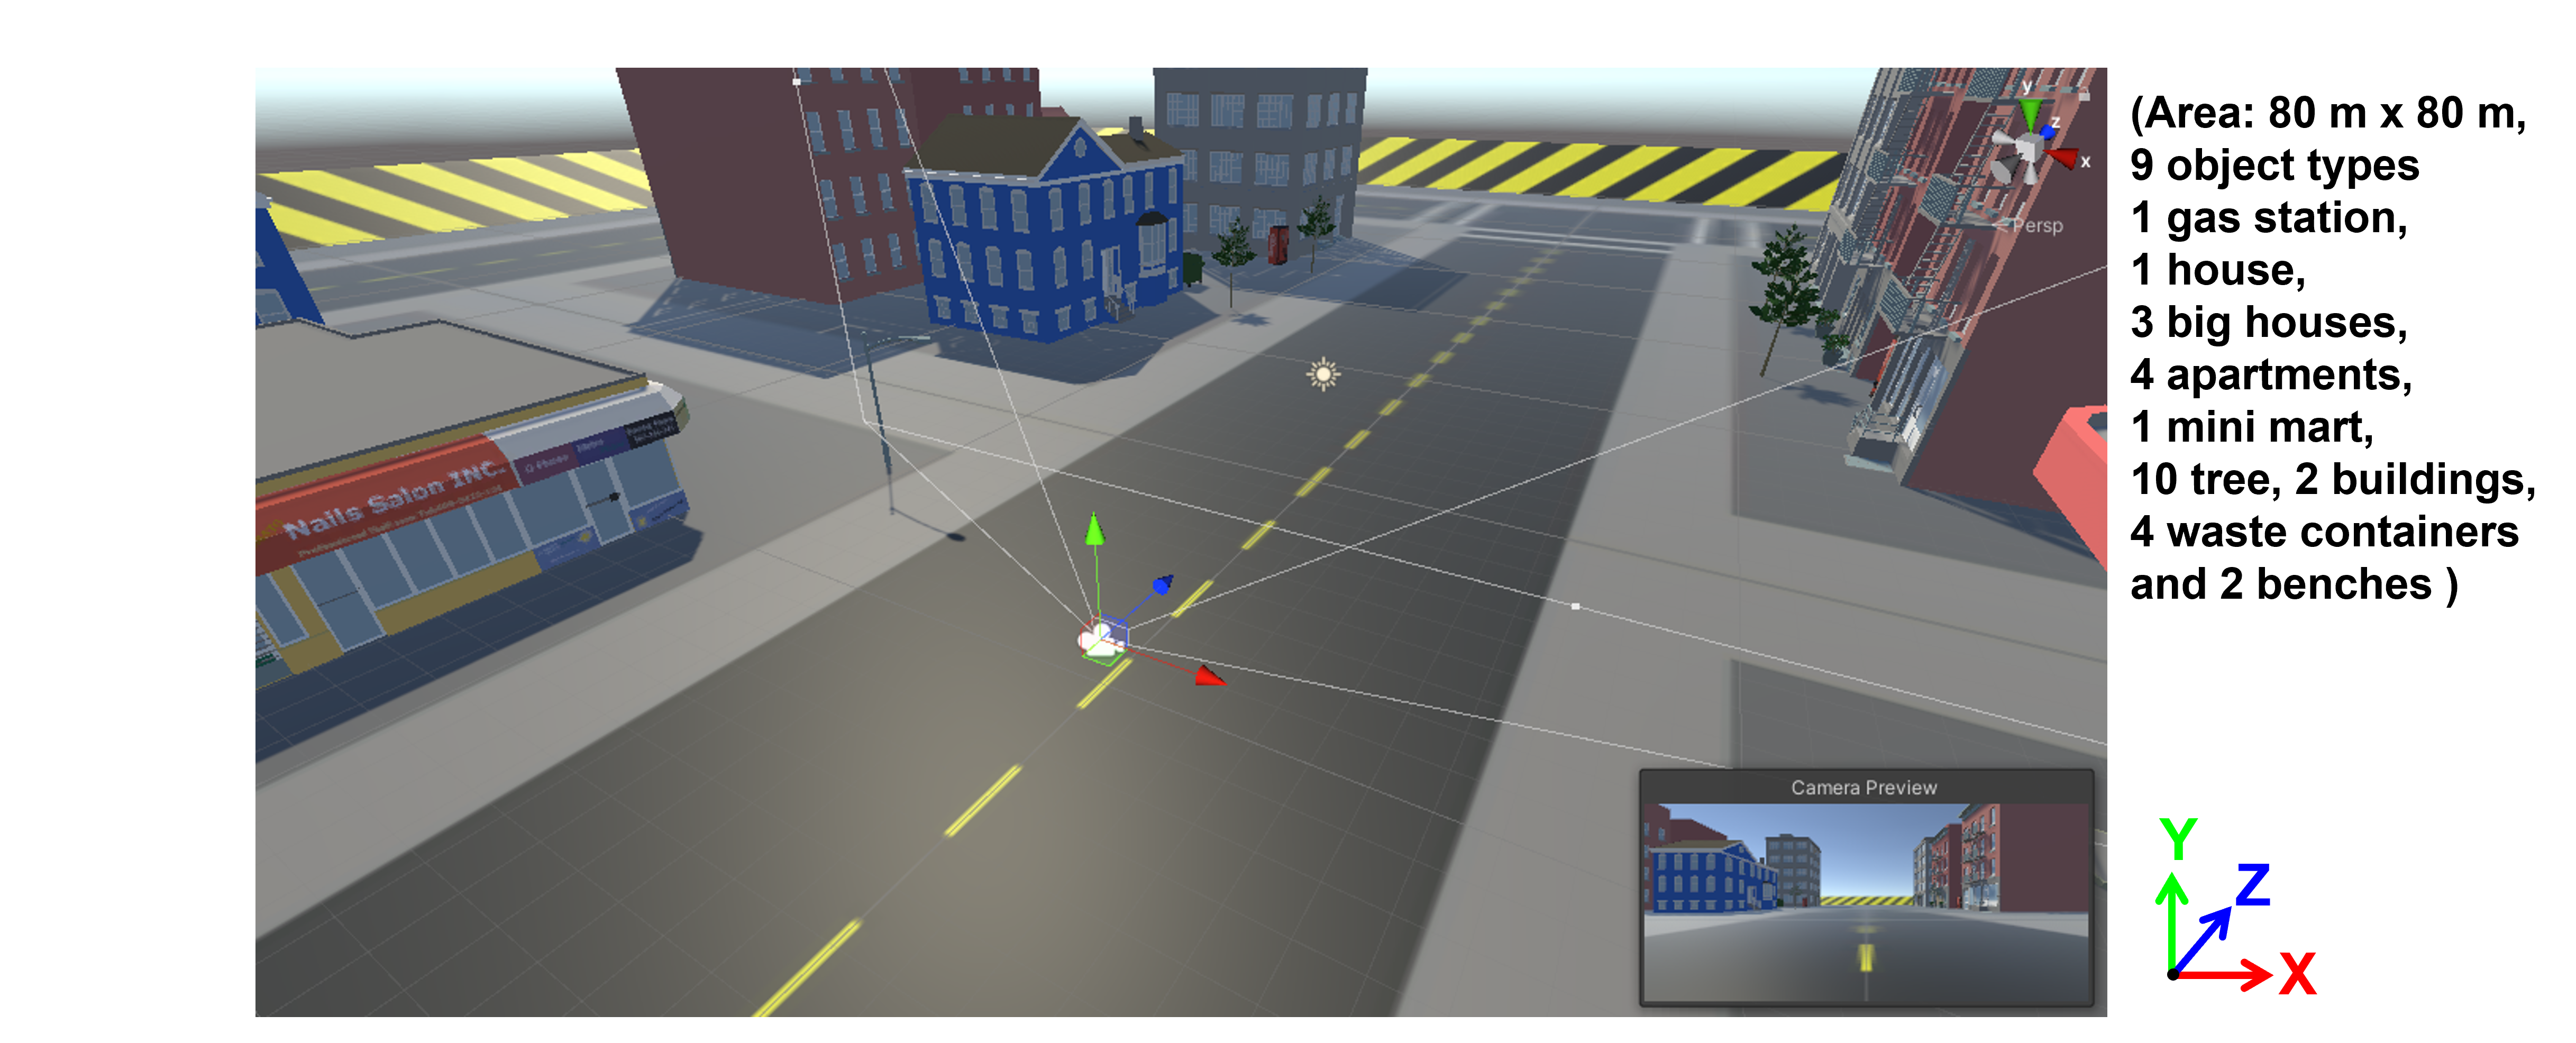
\includegraphics[width=1.1\textwidth]{Pictures/siteView.png}%imagine location
	\caption{A virtual environment from side view.}\label{fig:sideView}%use name for ref.
\end{figure}
\newpage

To realize a visual effect of rotating a virtual environment, relative rotation is applied to a virtual camera of the user, independently of his/her own rotation.

The stop to constant speed rotation task examines degree of sensitivity of humans' rotational awareness for a sudden start to the given speed. The subject puts on an HMD, then a randomly selected rotation speed (0.4deg/s, 0.8deg/s, 1.6deg/s, 3.2deg/s, 6.4deg/s and 12.8deg/s) is applied to the HMD coordinates. The subject is asked to press the button when he/she becomes aware of the rotation and the elapsed time is recorded. After that, the randomly selected speed for next is applied and the procedure is repeated.

\begin{figure}[H]\centering
	\includegraphics[width=1.0\textwidth]{Pictures/Equipment 1 Constant Speed task.png}%imagine location
	\caption{Stop to constant speed rotation task.}\label{fig:Equipment 1 Constant Speed task}%use name for ref.
\end{figure}
\newpage
%%%%%%%%%%%%%%%%%%%

The constant speed to stop rotation task examines degree of sensitivity of humans' rotational awareness for a sudden stop from given constant rotation speed. The subject puts on an HMD, HMD coordinates are then the rotated by a randomly selected constant speed (0.4deg/s, 0.8deg/s, 1.6deg/s, 3.2deg/s, 6.4deg/s and 12.8deg/s) at the beginning. This rotation stops without notice to the subject. The subject is asked to press the button when he/she becomes aware of the changing and the elapsed time is recorded. After that, the randomly selected speed for next is applied and the procedure is repeated.

In stop to constant speed and constant speed to stop rotation tasks, the direction of rotation is clockwise.

%%%%%%%%%%%%%%%%%%
\begin{figure}[H]\centering
	\includegraphics[width=1.0\textwidth]{Pictures/ConstantToStop.png}%imagine location
	\caption{Constant speed to stop rotation task.}\label{fig:Constant Speed to Stop Rotation task task}%use name for ref.
\end{figure}
\newpage


The deceleration rotation task examines degree of sensitivity of humans' awareness for a gradual change in speed of rotation. In this task, the HMD coordinates are rotated at the given constant speed (0.4deg/s, 0.8deg/s, 1.6deg/s and 3.2deg/s) when starting. And that speed is gradually decreased by a randomly selected deceleration (33\%, 66\% and 100\%). The $x$\% deceleration means that $x$\% of the given constant speed decreases per second until the speed reaches zero. The subject is asked to press the button when he/she becomes aware of the decrease in rotation speed and the elapsed time is recorded. After that, the randomly selected combination, speed and deceleration, is applied for next and procedure is repeated

Note that from the constant speed tasks, rotation speeds of 6.4deg/s and 12.8deg/s are high rotation speeds, so that the subjects suddenly responded after enabling or disabling rotation. For the deceleration and acceleration tasks, these speeds are excluded.

\begin{figure}[H]\centering
	\includegraphics[width=1.0\textwidth]{Pictures/Deceleration Task.png}%imagine location
	\caption{Deceleration rotation task.}\label{fig:Equipment 1 Deceleration Task}%use name for ref.
\end{figure}

\newpage
The acceleration rotation task examines degree of sensitivity of humans' awareness for a gradual increase in speed of rotation.
The initial rotation speed is zero, and a randomly selected rotation speed (0.4deg/s, 0.8deg/s, 1.6deg/s and 3.2deg/s) and a randomly selected acceleration (33\%, 66\% and 100\%) are applied to the HMD coordinates. Here, acceleration of $x$\% indicates that rotation speed increases by $x$\% of the given constant speed per second from zero until the speed reaches it. The subject is asked to press the button when he/she becomes aware of the rotation and the elapsed time is recorded. After that, the randomly selected combination, speed and acceleration, is applied for next and the procedure is repeated.

In deceleration and acceleration rotation tasks, the direction of rotation is clockwise. Fig.~\ref{fig:Equipment 1 Deceleration Task}, the blue arrow is a constant speed. The red arrow is deceleration rotation, and the arrow color is fading from dark red to bright red, which means the rotation speed decreases to zero. Fig.~\ref{fig:Equipment 1 Acceleration Task} shows the acceleration rotation task. The rotation speed is increasing, shown by fading color from bright red to dark red of the red arrow.

\begin{figure}[H]\centering
	\includegraphics[width=0.9\textwidth]{Pictures/Equipment 1 Acceleration Task.png}%imagine location
	\caption{Acceleration rotation task.}\label{fig:Equipment 1 Acceleration Task}%use name for ref.
\end{figure}
\newpage
\subsection{Procedure} 
Five subjects with the ages of 25 to 27 years old take part in the experiment.
\begin{enumerate}
	\item Each subject wears an HMD.
	\item A rotation speed (0.4deg/s, 0.8deg/s, 1.6deg/s, 3.2deg/s, 6.4deg/s and 12.8deg/s) and a percentage of acceleration or deceleration (33\%,66\% and 100\%) are randomly selected.
	\item The participant performs the given task (The first task is the stop to constant speed rotation task. The second task is the constant speed to stop rotation task, the third task is the deceleration rotation task and the final task performs the acceleration rotation task. Each task is performed on a different day.).
	\item Repeat from step 2 to step 3 at ((6 speeds x 3 trials x 2 tasks) + (4 speeds x 3 percentages x 3 trials x 2 tasks) = 108 trials)
\end{enumerate}

The subjects can take a break every 5 minutes to check VR motion sickness symptoms as shown in Fig.~\ref{fig:Virtual reality sickness questionnaire_1}.
\begin{figure}[H]\centering
	\includegraphics[width=1.0\textwidth]{Pictures/Virtual reality sickness questionnaire.png}%imagine location
	\caption{Virtual reality sickness questionnaire~\cite{Norman2018EvaluationOV}.}\label{fig:Virtual reality sickness questionnaire_1}%use name for ref.
\end{figure}
\newpage
\subsection{Data collection}
For each task, the following data is collected.

\begin{table}[h!]\centering
	\caption{Data collection.}
	\label{tab:Data CollectionEx1}%\scriptsize
		\scalebox{1.0}{
	\begin{tabular}{ |p{4cm}|p{3cm}|p{6cm}|}
	\hline
		Variable & Unit & Description \\\hline
		Elapsed time & second & Time to be aware.\\\hline
		Rotation speed & deg/second & Rotation speed of the coordinates of an HMD.\\\hline
		Acceleration (for acceleration rotation task) or deceleration (for deceleration rotation task) & percentage & Degree of accelerate or deceleration of the rotation speed.\\\hline
		
	\end{tabular}
	}
\end{table} 

Independent variables are Rotation speed and Acceleration or deceleration while a dependent one is Elapsed time.
\newpage
\subsection{Equipment}
The experiment system is developed on the Unity platform. The version of Unity is 2019.4.17f1. In terms of hardware, an HMD is served by HTC VIVE Cosmos (Fig.~\ref{fig:EquipmentAndSpecification}), which has a resolution of 1080x1200 pixels per eye, a diagonal field of view of roughly 110 degrees, and a frame rate of 90Hz. Two base stations included with HTC Vive are used for positional tracking, shown in Fig.~\ref{fig:Equipment1_AndSpecification}.

The HMD is connected to a computer with a CPU of Core i7 (8 cores), a GPU of NVIDIA GeForce GTX 1650 Super and a memory of 16GB.
\begin{figure}[H]\centering
	\includegraphics[width=0.6\textwidth]{Pictures/EquipmentAndSpecification.png}%imagine location
	\caption{Equipment and specification.}\label{fig:EquipmentAndSpecification}%use name for ref.
\end{figure}
\begin{figure}[H]\centering
	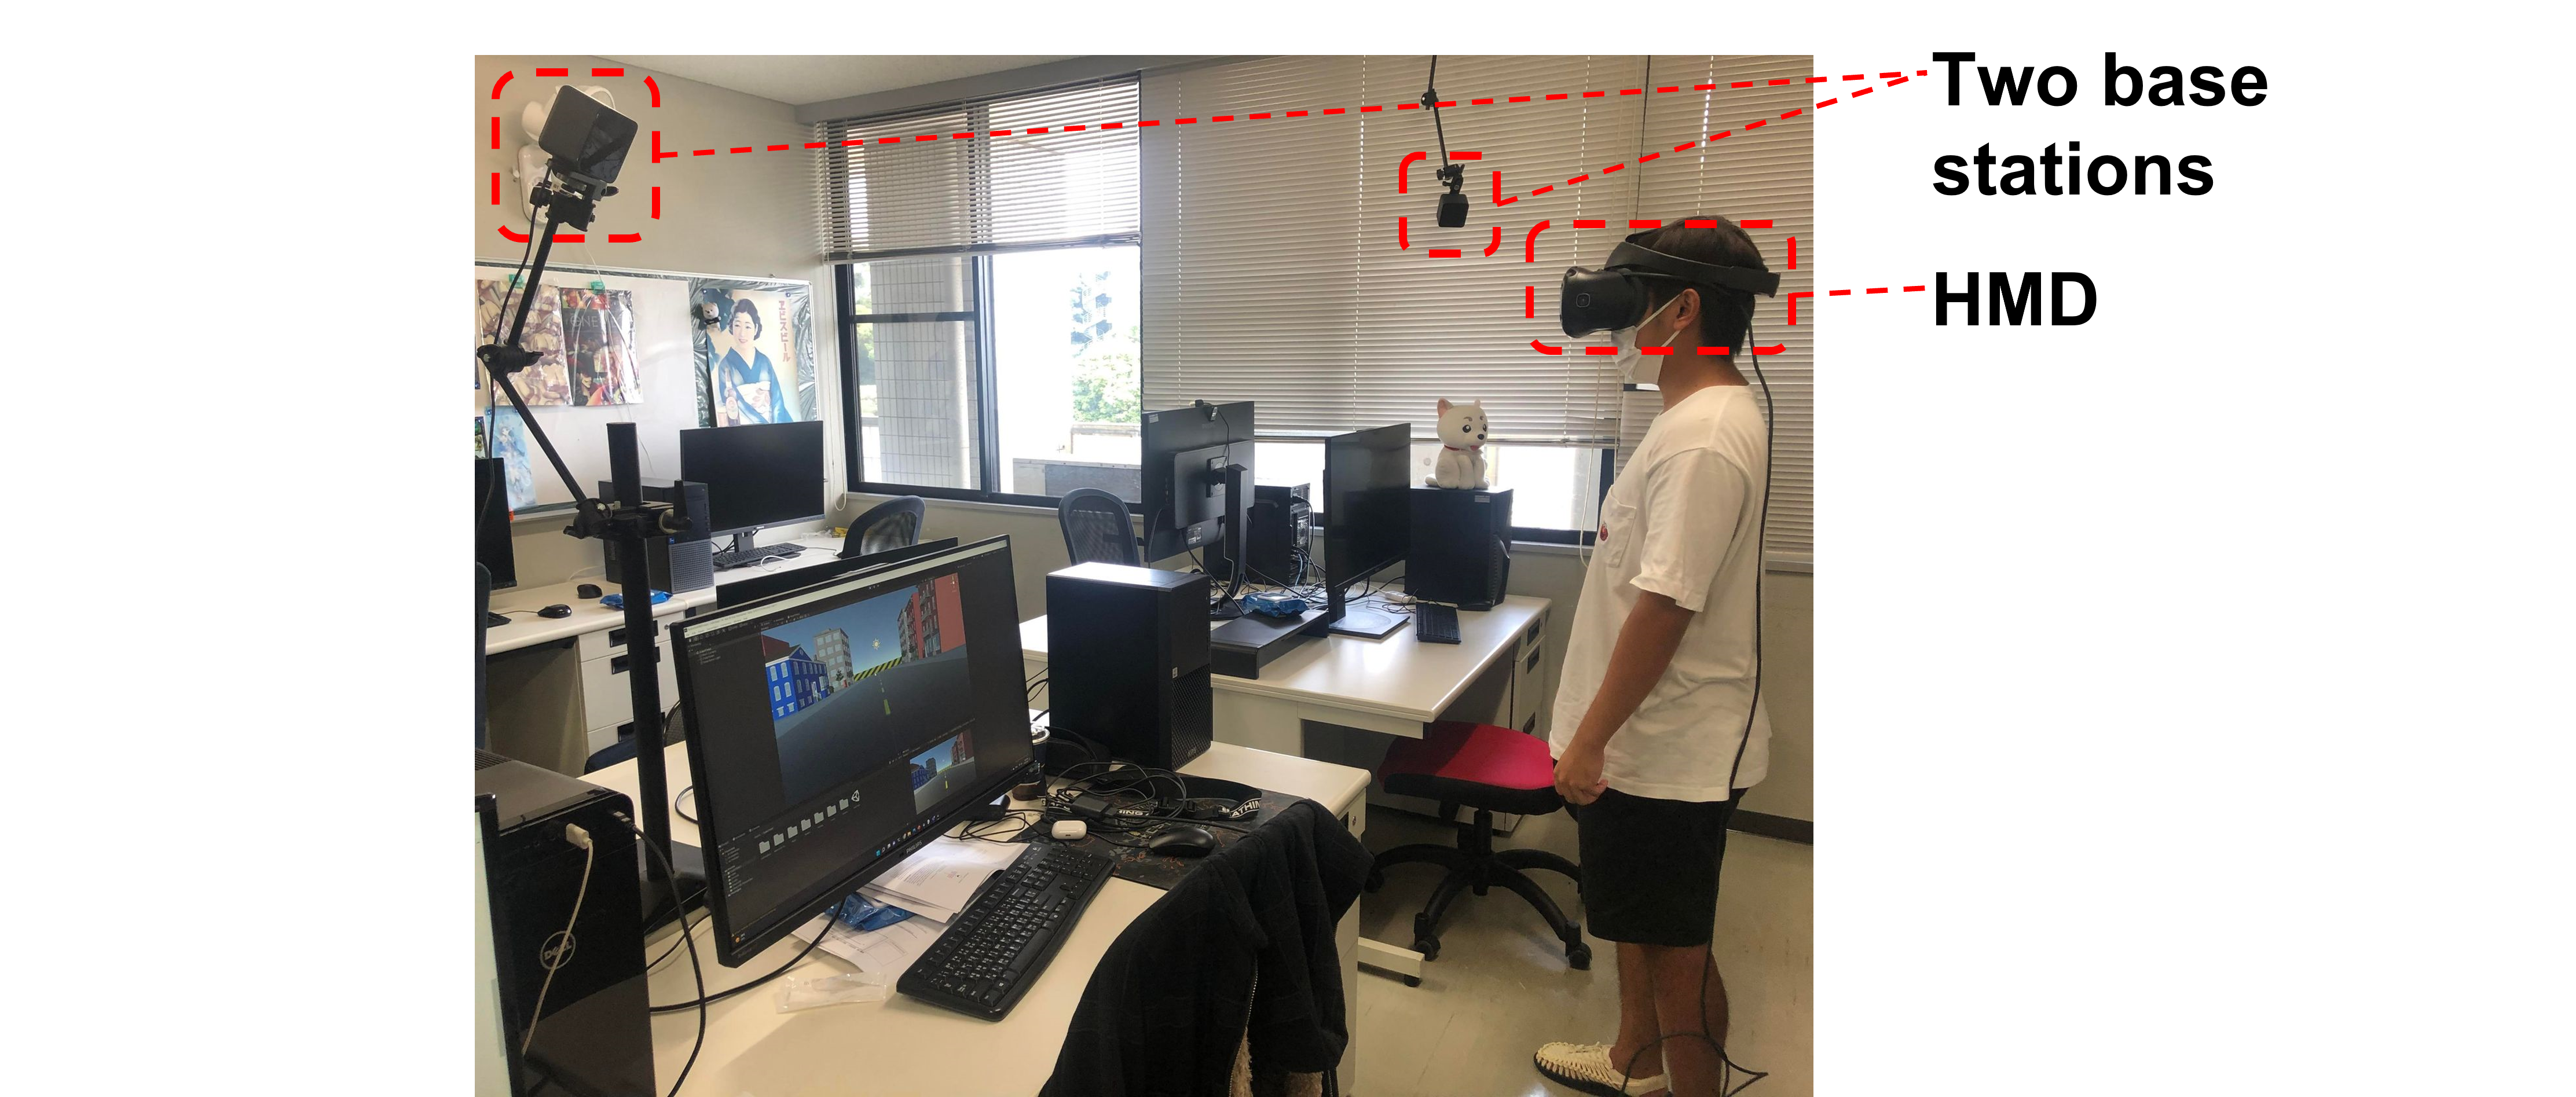
\includegraphics[width=1.2\textwidth]{Pictures/Experiment1_Overview.png}%imagine location
	\caption{A scene of the experiment.}\label{fig:Equipment1_AndSpecification}%use name for ref.
\end{figure}
\newpage
\subsection{Results}
Fig.~\ref{fig:Six constant speeds} shows a relationship between constant rotation speeds and the elapsed time to notice for the stop to constant speed rotation task. From the figure, when a rotation speed is slower than 0.8deg/s, it will take 10s for users to notice.

Fig.~\ref{fig:Stop to Six constant speeds} shows a relationship between constant rotation speeds and the elapsed time to notice for the constant speed to stop rotation task. From the result, a rotation speed is 0.4deg/s, the average elapsed time to notice is 7.72s.

Fig.~\ref{fig:Three deceleration of rotation} shows the impact of deceleration in rotation speed on the elapsed time. As the level of deceleration becomes smaller, it will take more time for users to notice. When a percentage of 33\%, subjects are going to take a long time to notice the rotation. The average elapsed time to notice at 33\% are 9.48s, 4.388s, 3.578s and 1.942s for the max rotation speed of 0.4deg/s, 0.8ged/s, 1.6deg/s and 3.2deg/s, respectively.

Fig.~\ref{fig:Three acceleration of rotation} shows the impact of acceleration in rotation speed on the elapsed time. As the level of acceleration becomes smaller, it will take more time for users to notice. When a percentage of 33\%, subjects are going to take a long time to notice the rotation. The average elapsed time to notice at 33\% are 14.57s, 14.106s, 8.818s and 2.926s for the max rotation speed of 0.4deg/s, 0.8deg/s, 1.6deg/s and 3.2deg/s, respectively.
\newpage
\begin{figure}[H]\centering
	\includegraphics[width=0.8\textwidth]{Pictures/Six constant speeds.png}%imagine location
	\caption{Results for stop to constant speed rotation task.}\label{fig:Six constant speeds}%use name for ref.
	
\end{figure}
\begin{figure}[H]\centering
	\includegraphics[width=0.8\textwidth]{Pictures/Stop to Six constant speeds.png}%imagine location
	\caption{Results for constant speed to stop rotation task.}\label{fig:Stop to Six constant speeds}%use name for ref.
	
\end{figure}
\begin{figure}[H]\centering
	\includegraphics[width=0.8\textwidth]{Pictures/Curvature distance for three decelerations at each constant speed.png}%imagine location
	\caption{Results for impact of deceleration of rotation on elapsed time.}\label{fig:Three deceleration of rotation}%use name for ref.
	
\end{figure}
\begin{figure}[H]\centering
	\includegraphics[width=0.8\textwidth]{Pictures/Three acceleration of rotation.png}%imagine location
	\caption{Results for impact of acceleration of rotation on elapsed time.}\label{fig:Three acceleration of rotation}%use name for ref.
	
\end{figure}


\newpage
%%%%%%%%%%%%%%%%%%%%%%%%%%%%%%%%%%%%%%%
%%%%%%%%%%%%%%%%%%%%%%%%%%%%%%%%%%%%%%%
\section{Curvature distance of humans walking in a rotating virtual environment}
When multiple users share the same physical space, they might collide. To prevent it, time-dependent synced-rotational gains are applied to the coordinates of their virtual environments so that they would walk in a curved path to away from the collision.

For properties of the curved path, the purpose of this experiment is to figure out the relation between applied rotational gains and their influence on the curved path.

\subsection{Curvature distance}
A curvature distance~\cite{6200791} is the right-angle distance from the straight line to a curved path(Fig.~\ref{fig:CurevDistance}). While a user is walking, the coordinates of his/her HMD will rotate to have him/her walk on a curved path to avoid the collision with other users.
\begin{figure}[H]\centering
	\includegraphics[width=0.9\textwidth]{Pictures/Curvature distance.png}%imagine location
	\caption{Curvature distance.}\label{fig:CurevDistance}%use name for ref.
\end{figure}

The required curvature distance to swerve the other user coming towards you is the average of half the width of a human shoulder~\cite{9660069}. The half the shoulder width is 23cm.

\newpage
\subsection{Experiment tasks}
In this experiment, two tasks are employed: constant speed task and acceleration task. The constant speed task examines susceptibility of humans' sense of direction to a constant speed of rotation.
The subject puts on an HMD, then a randomly selected rotation speed (0.4deg/s, 0.8deg/s, 1.6deg/s and 3.2deg/s) is applied to the HMD coordinates while the subject is walking for a specified distance. 

The acceleration task examines susceptibility of humans' sense of direction to a gradual increase in speed of rotation.
The initial rotation speed is zero, and a randomly selected rotation speed (0.4deg/s, 0.8deg/s, 1.6deg/s and 3.2deg/s) and a randomly selected acceleration (33\%, 66\% and 100\%) are applied to the HMD coordinates while the subject is walking for a specified distance. Fig.~\ref{fig:Equipment 2} shows a photo taken during the experiment. 
\begin{figure}[H]\centering
	\includegraphics[width=0.4\textwidth]{Pictures/Equipment 2.png}%imagine location
	\caption{A scene of the experiment.}\label{fig:Equipment 2}%use name for ref.
\end{figure}
\newpage

\subsection{Procedure} 
Five subjects with the ages of 25 to 27 years old take part in the experiment.
\begin{enumerate}
	\item Each subject wears an HMD.
	\item A rotation speed (0.4deg/s, 0.8deg/s, 1.6deg/s and 3.2deg/s) and a percentage of acceleration (33\%,66\% and 100\%) are randomly selected. 
	\item The subject performs the given task (The first task performs the constant speed
	task and the second task is the acceleration task).
	\item The subject is walking forward for 2 meters at 0.5m/s (the user's walking steps are prescribed by beep sounds)
	\item Repeat from step 2 to step 3 at ((4 constant speed x 3 trials) + (4 speed x 3 percentage x 3 trials) = 48 trials)
\end{enumerate}


The subjects can take a break every 5minutes to check VR motion sickness symptoms as show in Fig.~\ref{fig:Virtual reality sickness questionnaire_1}.



\subsection{Data collection}
For each task, the following data is collected.

\begin{table}[h!]\centering
	\caption{Data collection.}
	\label{tab:Data CollectionEx2}%\scriptsize
		\scalebox{1.0}{
	\begin{tabular}{ |p{4cm}|p{3cm}|p{6cm}|}
	\hline
		Variable & Unit & Description \\\hline
		Curvature distance & centimeter & The right-angle distance of the curvature of the real path relative to the virtual path.\\\hline
		Rotation speed & deg/second & Rotation speed of the coordinates of an HMD.\\\hline
		Acceleration (for acceleration task) & percentage & Degree of acceleration of the rotation speed.\\\hline
		
	\end{tabular}
	}
\end{table} 

Independent variables are Rotation speed and Acceleration while a dependent one is Curvature distance.




\newpage

\subsection{System environment}
Fig.~\ref{fig:Base State mapping area} shows the top view of a physical space where subjects walk in the experiment. The coordinates of the physical space are defined by two base stations whose positions are known, and the user’s position is tracked and stored in real time.

By considering the XZ plane, Fig.~\ref{fig:Walking Area in VR} shows the corresponding virtual environment in the experiment where the user moves. The path from the center to the each green box is on the X-axis or Z-axis. The relation between the distance in the virtual environment and the distance in the physical space is one-to-one correspondence.

\begin{figure}[H]\centering
	\includegraphics[width=0.7\textwidth]{Pictures/Base State mapping area.png}%imagine location
	\caption{Top view of a physical space used in the experiment.}\label{fig:Base State mapping area}%use name for ref.
\end{figure}
\begin{figure}[H]\centering
	\includegraphics[width=0.7\textwidth]{Pictures/Walking Area in VR.png}%imagine location
	\caption{A walking space in a virtual environment.}\label{fig:Walking Area in VR}%use name for ref.
\end{figure}

\newpage
\subsection{Results}
Fig.~\ref{fig:Curvature distance for four constant speeds} shows a relation between the obtained curvature distance and the given rotation speed. From the figure, the more rotation speed is added the more curvature distance is seen. When the rotation speed is increasing by 1deg/s, the curvature increase around 5.75cm.

Fig.~\ref{fig:Curvature distance for three accelerations at each constant speed} shows an impact of acceleration in rotation speed on curvature distance. At the degree of acceleration becomes smaller, the curvature distance will decrease a certain amount. When acceleration is increasing by 1\%, the curvature distance will increase by 0.0549cm on average.




\begin{figure}[H]\centering
	\includegraphics[width=0.8\textwidth]{Pictures/Curvature distance for four constant speeds.png}%imagine location
	\caption{Relation between curvature distance and rotation speeds.}\label{fig:Curvature distance for four constant speeds}%use name for ref.
	
\end{figure}


\begin{figure}[H]\centering
	\includegraphics[width=0.8\textwidth]{Pictures/Curvature distance for three accelerations at each constant speed.png}%imagine location
	\caption{Relation between curvature distance and acceleration of rotation speeds.}\label{fig:Curvature distance for three accelerations at each constant speed}%use name for ref.
	
\end{figure}


\begin{figure}[H]\centering
	\includegraphics[width=0.9\textwidth]{Pictures/edit.png}%imagine location
	\caption{Result between sensitivity of rotational awareness of humans (blue line) and curvature distance of humans walking (red line) in VR.}\label{fig:Exp2_Conclude}%use name for ref.
	
\end{figure}

Fig.~\ref{fig:Exp2_Conclude} shows a condition to perform the proposed method where a user is not aware of the rotation, and he/she swerves by half the shoulder width. The horizontal axis shows the rotation speed of the virtual environment in degrees per second and the horizontal one does the elapsed time in second. The blue line represents the elapsed time on average users spend until they become aware of rotation for each rotation speed. The red one represents the elapsed time on average users spend until they make 23cm of the curvature distance at the walking speed of 0.5m/s for each rotation speed. The red line is calculated from the values from Fig.~\ref{fig:Curvature distance for four constant speeds}. From the two lines, users can not avoid a collision without awareness of rotation because the time it takes to be aware of rotation is shorter than the time it takes to make the curvature distance of 23cm.

\newpage
\begin{figure}[H]\centering
	\includegraphics[width=1.0\textwidth]{Pictures/CurvatureDistanceandTimes.png}%imagine location
	\caption{Result between Sensitivity of Rotational Awareness of Humans (solid line) and Curvature Distance of Humans Walking (dash line) in VR.}\label{fig:Exp2_ConcludeOfacceration}%use name for ref.
\end{figure}

Fig.~\ref{fig:Exp2_ConcludeOfacceration} shows a condition to perform the proposed method where a user swerves by half the shoulder width while being unaware of it for each acceleration. The horizontal axis is the max rotation speed of the virtual environment, to which the rotation speed increases from zero. The horizontal axis is the elapsed time in second. For each max rotation speed, the solid line shows the average amount of time it takes for users to become aware of rotation with acceleration. The dashed line shows how long it takes for users to cover 23cm of the curvature distance at a speed of 0.5m/s for each max rotation speed. The solid line and the dashed line are calculated from Fig.~\ref{fig:Three acceleration of rotation} and Fig.~\ref{fig:Curvature distance for three accelerations at each constant speed}. The gray line presents an acceleration of 33\%, the orange line presents an acceleration of 66\%, and the blue line gives an acceleration of 100\%. From these results, the proposed method is capable of having users swerve by half the shoulder 23cm without awareness of rotation at the max rotation speed of 1.6 deg/s and acceleration of 100\% at the duration of about 8 seconds.


